\section{Data-Generating Process}

The benchmark generator is the discrete-time stochastic map
\begin{equation}
  x_{t+1}=x_t+\sin(x_t)\Delta t+\sqrt{D}\varepsilon_t,
\end{equation}
where the initial state is close to zero and \(\sin(x_t)\) gives a nonlinear
periodic drift. The innovation sequence \(\varepsilon_t\) is generated for a
fixed length, centered, and scaled to unit empirical variance when possible.
The map is motivated by stochastic dynamics, but it is not treated as a strict
Euler--Maruyama discretization of a continuous-time diffusion: the
implementation applies the \(\sqrt{D}\) factor shown above and does not add a
separate \(\sqrt{\Delta t}\) factor. Thus \(D\) controls the perturbation scale
of this discrete benchmark source.

Colored innovations are generated by Fourier-domain spectral shaping of a
Gaussian white sequence \cite{timmer1995,kasdin1995}. For a length-\(N\) draw,
the real Fourier transform \(Z_k\) is multiplied by
\begin{equation}
  a_c(f)=
  \begin{cases}
    1, & \text{white},\\
    f^{-1/2}, & \text{pink},\\
    f^{-1}, & \text{Brownian/red},\\
    f, & \text{violet},\\
    f^{1/2}, & \text{blue},
  \end{cases}
  \qquad f>0 .
\end{equation}
The zero-frequency component is not used for singular colored families. The
weights are normalized by their root mean square before the inverse transform;
the real sequence is then centered and scaled. Thus the innovation family
controls temporal correlation, not empirical variance scale.

\subsection{Transition Labels}

Change points in this benchmark are event labels, not parameter breaks in the
generator. Let \(L_t\) denote the integer level assigned to \(x_t/\pi\) by the
canonical level-mapping rule. The binary label at time \(t\) is one when
\(L_t \ne L_{t-1}\) and zero otherwise. The same stochastic map therefore
generates the whole path, while the level-crossing rule converts that path into
transition-time labels. A rule that directly recomputes \(L_t\) from \(x_t\)
would reproduce the annotation mechanism; it is not treated as a competing CPD
detector. The compared methods are evaluated as general-purpose detectors
applied to the trajectory without using the precomputed level sequence.

\begin{figure}[htbp]
  \centering
  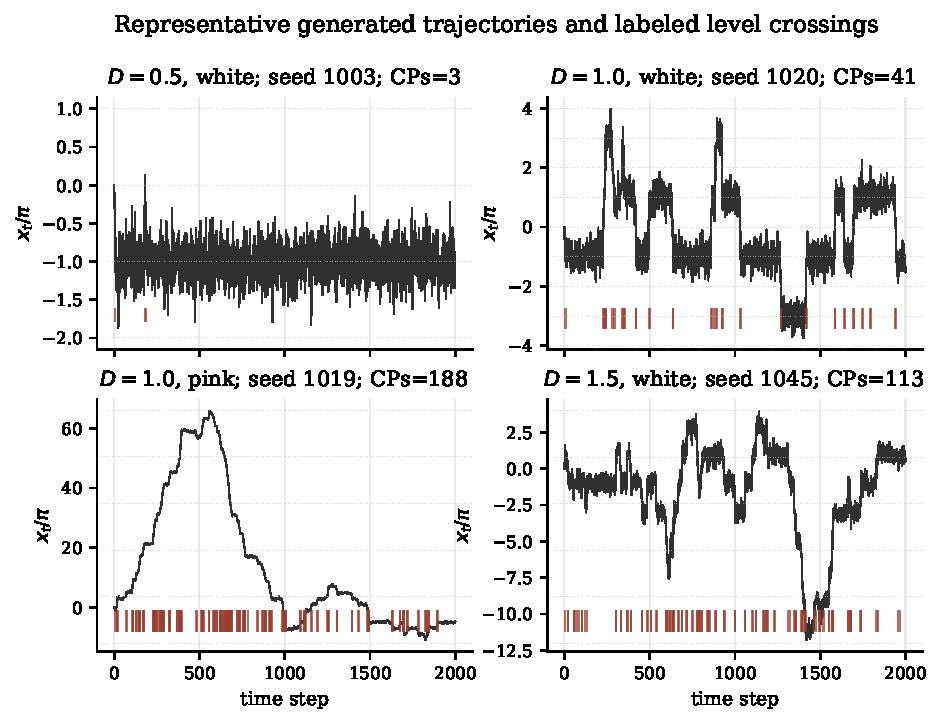
\includegraphics[width=\linewidth]{../assets/figures/fig01_generated_regime_examples.pdf}
  \caption{Representative trajectories and labeled level crossings under the
  four frozen benchmark scenarios. Red ticks indicate true labels; larger
  \(D\) or correlated innovations create denser transition neighborhoods.}
  \label{fig:generated-regime-examples}
\end{figure}

\subsection{Transition Properties}

The parameter \(D\) controls how often the trajectory leaves one level region.
In a diagnostic grid with \(\Delta t=1.0\), white innovations, length 10000,
and 30 series per setting, \(D=0.5\) produced 6.4 change points per series on
average, with mean positive holding time about 936 steps. For \(D=1.0\) and
\(D=1.5\), the corresponding values were about 197/50 and 576/17. Thus the
\(D=1.5\) case is dense relative to the 25-step matching tolerance and must be
read with the robustness check.

Because colored innovations change temporal correlation structure, colored-noise
comparisons are treated as separate experimental settings rather than direct
quantitative extensions of the white-noise cases.

The generator outputs \((x_{0:T}, y_{0:T})\), both of length \(T+1\), with
zero-based indexing. No-change cases use an all-zero label vector or an empty
change-point list. Reportable runs store the dataset source, generation
parameters \((T,\Delta t,D,\) noise type, seed\()\), and source path.

